右の図のように、1辺の長さが1の正三角形で、平面を分割する。これらの1辺の長さが1の正三角形1つ1つを、単位正三角形とよぶことにする。は
じめに1個以上有限個の単位正三角形が塗りつぶされているとし、以下の操作を繰り返すことにより、次々に単位正三角形を塗りつぶしていく。

『1回の操作ごとに、既に塗りつぶされている単位正三角形と少なくとも1つの辺を共有する単位正三角形を、すべて塗りつぶす』

次の問いに答えよ。

\begin{enumerate}
  \item はじめに塗りつぶされている単位正三角形が1つだけのとき、$n$回目の操作が終わったときに塗りつぶされている単位正三角形の個数 $a_n$ を求めよ。
  \item はじめに2個以上有限個の単位正三角形が塗りつぶされているとき、$n$回目の操作が終わったときに塗りつぶされている単位正三角形の個数を $b_n$ とおくと、極限
        \begin{align}
          \lim_{n \to \infty} \frac{a_n}{b_n}
        \end{align}
        は、はじめの塗りつぶされ方がどのようであっても存在するか。極限が存在する場合については、その極限値を求めよ。存在しない場合があるならば、その例をあげよ。
\end{enumerate}

\begin{figure}[H]
  \centering
  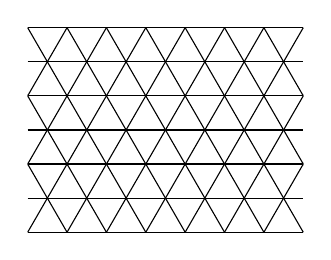
\begin{tikzpicture}[scale=0.5]
    % Drawing triangular grid
    % Drawing triangular grid with equilateral triangles
    \clip (-0.5,0) rectangle (6.5,0.866*6);

    \foreach \i in {0,...,6} {
        % Horizontal lines
        \draw (-0.5, {0.866*\i}) -- (6.5, {0.866*\i});
      }
    \foreach \k in {-4,...,10} {
        % 斜め線
        \draw ({-0.5+\k}, 0) -- ({-0.5+\k - 0.5*6}, {0.866*6});  % 傾き60度（右上がり）
        \draw ({-0.5+\k}, 0) -- ({-0.5+\k + 0.5*6}, {0.866*6}); % 傾き120度（左上がり）
      }
  \end{tikzpicture}
\end{figure}
